\subsection{角的比较和度量}\label{subsec:czjh1-1-6}

在小学我们学过,角是有大小的。怎样比较两个角的大小呢?我们先做一个实验。
如图 \ref{fig:czjh1-1-26} 那样,将两块三角板叠放在一起,使要比较的两个角的顶点和一边分别对齐,
这时,我们可以看到,在图 \ref{fig:czjh1-1-26} 甲中,两角的另一边也叠合在一起;
而在图 \ref{fig:czjh1-1-26} 乙中,两角的另一边是不叠合在一起的。
这样就可以比较出两个角的大小了。比较两个角的大小,和上面的方法相同。

\begin{figure}[htbp]
    \centering
    \begin{minipage}[b]{7cm}
        \centering
        \begin{tikzpicture}
	\pgfmathsetmacro{\r}{0.3}

	\pgfmathsetmacro{\ab}{2}
	\pgfmathsetmacro{\ac}{\ab * sqrt(3)}
	\tkzDefPoints{0/0/A, \ab/0/B, 0/\ac/C}
	\tkzDefMidPoint(B,C)    \tkzGetPoint{a}
	\tkzDefMidPoint(A,C)    \tkzGetPoint{b}
	\tkzInterLL(A,a)(B,b)   \tkzGetPoint{O}
	\tkzDefCircle[R](O,\r)  \tkzGetPoint{o}
	\tkzDrawPolygon(A,B,C)
	\tkzDrawCircle(O,o)
	\tkzMarkAngle[size=0.3](B,A,C)

	\pgfmathsetmacro{\nab}{2.5}
	\tkzDefPoints{0/0/nA, \nab/0/nB, 0/\nab/nC}
	\tkzDefMidPoint(nB,nC)      \tkzGetPoint{na}
	\tkzDefMidPoint(nA,nC)      \tkzGetPoint{nb}
	\tkzInterLL(nA,na)(nB,nb)   \tkzGetPoint{nO}
	\tkzDefCircle[R](nO,\r)      \tkzGetPoint{no}
	\tkzInterLL(nB,nC)(B,C)     \tkzGetPoint{M}

	%\tkzDrawPolygon(nA,nB,nC)
	\tkzDrawSegments(nA,nB  nA,nC  nB,M)
	\tkzDrawSegments[dashed](M,nC)

	\tkzDrawCircle[dashed](nO,no)
	\tkzMarkAngle[size=0.3](nB,nA,nC)
\end{tikzpicture}


        \caption*{甲}
    \end{minipage}
    \qquad
    \begin{minipage}[b]{7cm}
        \centering
        \begin{tikzpicture}
	\pgfmathsetmacro{\r}{0.3}

	\pgfmathsetmacro{\ab}{2}
	\pgfmathsetmacro{\ac}{\ab * sqrt(3)}
	\tkzDefPoints{0/0/B, \ab/0/A, \ab/\ac/C}
	\tkzDefMidPoint(B,C)    \tkzGetPoint{a}
	\tkzDefMidPoint(A,C)    \tkzGetPoint{b}
	\tkzInterLL(A,a)(B,b)   \tkzGetPoint{O}
	\tkzDefCircle[R](O,\r)  \tkzGetPoint{o}
	\tkzDrawPolygon(A,B,C)
	\tkzDrawCircle(O,o)
	\tkzMarkAngle[size=0.3](A,B,C)

	\pgfmathsetmacro{\nab}{2.5}
	\tkzDefPoints{0/0/nB, \nab/0/nA, \nab/\nab/nC}
	\tkzDefMidPoint(nB,nC)      \tkzGetPoint{na}
	\tkzDefMidPoint(nA,nC)      \tkzGetPoint{nb}
	\tkzInterLL(nA,na)(nB,nb)   \tkzGetPoint{nO}
	\tkzDefCircle[R](nO,\r)     \tkzGetPoint{no}
	\tkzInterLL(nB,nC)(A,C)     \tkzGetPoint{M}

	%\tkzDrawPolygon(nA,nB,nC)
	\tkzDrawSegments(nA,nB  nA,nC  nC,M)
	\tkzDrawSegments[dashed](M,nB)

	\tkzDrawCircle[dashed](nO,no)
	\tkzMarkAngle[size=0.5](nA,nB,nC)
\end{tikzpicture}


        \caption*{乙}
    \end{minipage}
    \caption{}\label{fig:czjh1-1-26}
\end{figure}

如图 \ref{fig:czjh1-1-27} , 把  $\angle AOB$ 放到 $\angle A'O'B'$ 上面,使顶点 $O$ 与 $O'$ 重合,
边 $OA$ 与 $O'A'$ 重合,另一边 $OB$ 与 $O'B'$ 在 $O'A'$ 的同旁。
这时,有下面三种可能情形;

{
    \def\baseabc{
        \tkzDefPoint(0,0){O}
        \tkzDefPoint(0:2){A}
        \tkzDefPoint(40:2){B}
        \tkzDrawSegments(O,A  O,B)
        \tkzLabelPoints[below](O, A)
        \tkzLabelPoints[right](B)
    }

    \def\comparedabc{
        \tkzDefPoint(0,0){O}
        \tkzDefPoint(0:2){A}
        \tkzDefPoint(40:2){B}
        \tkzDrawSegments(O,A  O,B)
        \tkzLabelPoint[below](O){$(O)$}
        \tkzLabelPoint[below](A){$(A)$}

        \tkzLabelPoint[above](O){$O'$}
        \tkzLabelPoint[above](A){$A'$}
    }
\begin{figure}[htbp]
    \centering
    \begin{minipage}[b]{4cm}
        \centering
        \begin{tikzpicture}
	\begin{scope}
		\baseabc
	\end{scope}

	\begin{scope}[yshift=-2.3cm]
		\comparedabc
		\tkzLabelPoint[right=1.3em](B){$(B)$}

		\tkzLabelPoint[right](B){$B'$}
	\end{scope}
\end{tikzpicture}


        \caption*{甲}
    \end{minipage}
    \qquad
    \begin{minipage}[b]{4cm}
        \centering
        \begin{tikzpicture}
	\begin{scope}
		\baseabc
	\end{scope}

	\begin{scope}[yshift=-2.3cm]
		\comparedabc
		\tkzLabelPoint[right](B){$B$}

		\tkzDefPoint(55:2){B'}
		\tkzDrawSegment(O,B')
		\tkzLabelPoint[right](B'){$B'$}
	\end{scope}
\end{tikzpicture}


        \caption*{乙}
    \end{minipage}
    \begin{minipage}[b]{4cm}
        \centering
        \input{../pic/czjh1-ch1-27-c}
        \caption*{丙}
    \end{minipage}
    \caption{}\label{fig:czjh1-1-27}
\end{figure}
}

(1) 边 $OB$ 与 $O'B'$ 重合(图 \ref{fig:czjh1-1-27} 甲)。
这时,两个角相等,记作 $\angle AOB = \angle A'O'B'$。

(2) 边 $OB$ 落在 $\angle A'O'B'$ 的内部(图 \ref{fig:czjh1-1-27} 乙)。
这时,$\angle AOB$ 小于 $\angle A'O'B'$(或说 $\angle A'O'B'$ 大于 $\angle AOB$)。
记作 $\angle AOB < \angle A'O'B'$ (或 $\angle A'O'B' > \angle AOB$ )。

(3) 边 $OB$ 落在 $\angle A'O'B'$ 的外部(图 \ref{fig:czjh1-1-27} 丙),也就是说, $O'B'$ 在 $\angle AOB$ 的内部。
这时 $\angle AOB > \angle A'O'B'$(或 $\angle A'O'B' < \angle AOB$)。

在小学,我们曾用量角器来度量角,它的度量单位是度、分、秒。
把周角分成 $360$ 等份, 每一份是一度,记作 $1^\circ$;
每一度分成 $60$ 等份,每一份是一分,记作 $1'$;
每一分分成 $60$ 等份,每一份是一秒,记作 $1''$。

一个角的度数是 $48^\circ 56'  37''$, 读作 48 度 56 分 37 秒。
{\bfseries
\begin{align*}
    & \bm{1 \text{周角} = 2 \text{平角} = 360^\circ } \fenhao \\
    & \hspace*{4em} \bm{1 \text{平角} = 180^\circ } \fenhao \\
    & \bm{1^\circ = 60' \douhao \quad 1' = 60''} \juhao
\end{align*}}


\liti 用度、分、秒表示 $57.32^\circ$。

\jie 先把 $0.32^\circ$ 化为分:$60' \times 0.32 = 19.2'$;

再把 $0.2$ 化为秒: $60'' \times 0.2 = 12''$。

$\therefore$ \quad $57.32^\circ = 57^\circ 19' 12''$。


\begin{enhancedline}
\liti  用度表示 $10^\circ 23' 45''$。

\jie 先把 $45''$ 化为分: $45'' = \dfrac{1'}{60} \times 45 = 0.75'$;

再把 $23.75'$ 化为度: $23.75' = \dfrac{1^\circ}{60} \times 23.75 \approx 0.396^\circ$。

$\therefore$ \quad $10^\circ 23' 45'' \approx 10.396^\circ$。
\end{enhancedline}


\liti \begin{tblr}[t]{colsep=0pt, rowsep=0pt}
    计算: (1) $180^\circ - (35^\circ 18' + 62^\circ 56')$; \\
    (2) $32^\circ 16' \times 5$; (3) $15^\circ 20' \div 6$。
\end{tblr}


\jie (1) $180^\circ - (35^\circ 18' + 62^\circ 56') = 180^\circ - 98^\circ 14' = 81^\circ 46'$;

(2) $32^\circ 16' \times 5 = 160^\circ + 80' = 161^\circ 20'$;

(3) $15^\circ 20' \div 6 = 2^\circ + 200' \div 6 = 2^\circ 33' + 120'' \div 6 = 2^\circ 33' 20''$。


\begin{enhancedline}
\liti 由 2 点 30 分到  2 点 55 分,时钟的分针转了多大角度?

\jie 时钟表面共分成 12 大格,每格占周角的 $\dfrac{1}{12}$, 由 2 点 30 分到 2 点 55 分,分针共走了 5 格。

$\angle AOB = \dfrac{5}{12} \times 360^\circ = 150^\circ$。

答:分针转了 $150^\circ$ 角。
\end{enhancedline}

\begin{figure}[htbp]
    \centering
    \begin{minipage}[b]{7cm}
        \centering
        \includegraphics[width=3.5cm]{../pic/czjh1-ch1-28.png}
        \caption{}\label{fig:czjh1-1-28}
    \end{minipage}
    \qquad
    \begin{minipage}[b]{7cm}
        \centering
        
\begin{tikzpicture}
	\tkzDefPoints{0/0/O, 2/0/A, 2/3/B, 0/3/C}
	\tkzDrawSegments(O,A  O,B  O,C)
	\tkzMarkAngle[size=0.3](A,O,B)
	\tkzMarkAngle[size=0.53](B,O,C)
	\tkzLabelAngle[pos=0.5](A,O,B){$1$}
	\tkzLabelAngle[pos=0.8](B,O,C){$2$}

	\tkzLabelPoints[left](O)
	\tkzLabelPoints[right](A, B)
	\tkzLabelPoints[left](C)
\end{tikzpicture}


        \caption*{(第 1 题)}
    \end{minipage}
\end{figure}

\begin{lianxi}

\xiaoti{用量角器量图中 $\angle 1$ 和 $\angle 2$ 的度数(精确到 $1^\circ$), 并且计算出 $\angle AOC$ 的度数。}

\xiaoti{画直线 $AB$, 在 $AB$ 上任意取一点 $O$,并任意画射线 $OC$,
    用量角器量 $\angle AOC$ 的度数(精确到 $1^\circ$), 并且计算出 $\angle COB$ 的度数。
}


\xiaoti{用度、分、秒表示:(1) $33.33^\circ$; (2)$156.27^\circ$。}

\xiaoti{用度表示:(1)$50^\circ 40' 30''$; (2)$118^\circ 20' 42''$。}

\xiaoti{计算:}
\begin{xiaoxiaotis}

    \begin{tblr}{}
        \xxt{$37^\circ 28' + 44^\circ 49'$;} & \xxt{$108^\circ 18' - 50^\circ 00' 30''$;} \\
        \xxt{$25^\circ 36' \times 4$;}       & \xxt{$40^\circ 40' \div 3$。}
    \end{tblr}
\end{xiaoxiaotis}


\xiaoti{由 3 点整到 5 点 30 分,时钟的时针转了多大角度?}

\end{lianxi}

